\chapter{Narzędzia, architektura i implementacja}
\label{chap:algs}

\section{Narzędzia}

Silnik została napisany jako biblioteka w języku C w standardzie C11. Budowanie biblioteki ze źródeł wymaga generacji
dodatkowego kodu przy pomocy skryptów w języku Python w wersji 3.9.7.

Silnik został w całości opracowany na przy użyciu środowiska programistycznego CLion w wersji 2021.2.3.

Proces testowania i debugowania odbywał się na maszynie o następującej konfiguracji:
\begin{itemize}
	\item {OS}: Kubuntu 22.04.1 LTS x86-64,
	\item {CPU}: 11th Gen Intel Core i5-11400 (2.60GHz),
	\item {GPU}: Intel UHD Graphics 730 (Rocket Lake GT1).
\end{itemize}

Podczas pracy stosowano rozproszony system kontroli wersji git. Repozytorium jest utrzymywane na serwisie GitHub.

Pliki \textit{.clang-tidy} i \textit{.clang-format} znajdujące się w strukturze plików projektu pozwalają na automatyczne formatowanie
kodu źródłowego zgodnie ze uprzednio zdefiniowanym standardem kodowania.

Proces budowania projektu jest zautomatyzowany przy użyciu narzędzia CMake, które w przypadku języków C i C++ jest
praktycznie standardem podczas rozwoju wieloplatformowych projektów.

\subsection{Proces budowania}

Proces budowania silnika jest zdefiniowany w pliku *CMakeLists.txt* znajdującym się w katalogu głównym projektu.

Kompilacja kodu źródłowego w języku C jest obsługiwana bezpośrednio przez CMake, które generuje standardowe pliki
kompilacji (pliki Makefile w systemie Unix, projekty Microsoft Visual C++ w systemie Windows). Użyto prekompilowanych
nagłówków do przyśpieszenia kompilacji bibliotek zewnętrznych.

Skrypty w języku Python są obsługiwane pośrednio przez CMake, które wykrywa zainstalowany interpreter języka Python i
używa go do stworzenia tzw. środowiska wirtualnego w tymczasowym katalogu venv/ w głównym katalogu projektu. Podczas
procesu budowania środowisko wirtualne jest używane do zainstalowania wymaganych zewnętrznych bibliotek w języku Python
i wykonywania skryptów generatora kodu. Zaletą użycia środowiska wirtualnego w porównaniu do bezpośredniego wywoływania
zainstalowanego interpretera Pythona jest izolacja zarządzania zależnościami od reszty systemu operacyjnego, co pozwala
na łatwiejszą powtarzalność podczas debugowania \cite{PEP405}.

CMake organizuje proces budowania jako graf, w którym wierzchołki to cele połączonych ze sobą zależnościami. Budowa celu
wymaga wcześniejszego zbudowania wszystkich innych celów od których zależy budowany cel.

Wyróżniane są trzy rodzaje celów:
\begin{itemize}
	\item {plik wykonywalny}
	\item {biblioteka}: statyczna lub dynamiczna
	\item {cel niestandardowy}: używany do uruchamiania zewnętrznych programów podczas procesu kompilacji, np. generatorów kodu
\end{itemize}

Poniższy diagram przedstawia proces budowania projektu w formie celów i ich zależności:
\begin{figure}[H]
	\centering
	\begin{tikzpicture}[node distance=2cm]
		\tikzstyle{module} = [rectangle, rounded corners, minimum width=3cm, minimum height=1cm,text centered, draw=black]
		\tikzstyle{arrow} = [thick,->,>=stealth]
		
		\node (main) [module] {main};
		\node (test) [module, right = of main] {test};
		\node (assetpipeline) [module, right = of test] {asset\_pipeline};
		
		\node (engine) [module, below = of main] {engine};
		
		\node (runassetpipeline) [module, above = of assetpipeline] {run\_asset\_pipeline};
		\node (copyasset) [module, left = of runassetpipeline] {copy\_asset};
		
		\draw [arrow] (main) -- (engine);
		\draw [arrow] (test) edge[out=180, in=45] (engine);
		\draw [arrow] (assetpipeline) edge[out=-90, in=0] (engine);
		
		\draw [arrow] (main) edge[]  (runassetpipeline);
		\draw [arrow] (test) edge[]  (runassetpipeline);
		
		\draw [arrow] (runassetpipeline) -- (assetpipeline);
		
		\draw [arrow] (main) -- (copyasset);
		\draw [arrow] (test) -- (copyasset);
		\draw [arrow] (assetpipeline) -- (copyasset);
		\draw [arrow] (runassetpipeline) -- (copyasset);
		
		\node(plikiwykonywalne)[draw,dotted,fit=(main) (test) (assetpipeline)] {};
		\node (plikiwykonywalneLabel)[below=0cm of plikiwykonywalne] {\textbf{Pliki wykonywalne}};
		
		\node(biblioteki)[draw,dotted,fit=(engine)] {};
		\node (bibliotekiLabel)[below=0cm of biblioteki] {\textbf{Biblioteki}};
		
		\node(celeniestandardowe)[draw,dotted,fit=(copyasset) (runassetpipeline)] {};
		\node (celeniestandardoweLabel)[above=0cm of celeniestandardowe] {\textbf{Cele niestandardowe}};
		
	\end{tikzpicture}
	\caption{Proces budowania w formie celów i ich zależności (opracowanie własne)}
	\label{cmake}
\end{figure}

\paragraph{engine} Cel budujący bibliotekę programistyczną zawierającą implementację silnika.

\paragraph{main} Cel budujący plik wykonywalny demonstujący użycie silnika poprzez wyrenderowanie przykładowej sceny.

\paragraph{test} Cel budujący plik wykonywalny z testami jednostkowymi napisanymi i używanymi podczas implementowania projektu.

\paragraph{asset\_pipeline} Cel budujący plik wykonywalny służący jako narzędzie wiersza poleceń wykonujące operacje potoku zasobów.

\paragraph{copy\_assets} Niestandardowy cel kopiujący podkatalogu głównego \textit{assets} zawierającego nieprzetworzone zasoby wejściowe do katalogu budowania.

\paragraph{run\_asset\_pipeline} Niestandardowy cel realizujący potoku zasobów poprzez uruchomienie skryptu Python wielokrotne uruchamiającego narzędzie \textbf{asset\_pipeline} na zasobach wejściowych.


\subsection{Biblioteki zewnętrzne}

Projekt używa następujących zewnętrznych bibliotek programistycznych:

\begin{itemize}
	\item {\textit{Vulkan SDK 1.3.211.0}}:
	\begin{itemize}
		\item pliki nagłówkowe dla Vulkan,
		\item \textit{shaderc}: kompilacja shaderów z kodu źródłowego GLSL do kodu bajtowego SPIR,
		\item \textit{SPIRV-Reflect}: mechanizm refleksji dla kodu bajtowego SPIR-V,
	\end{itemize}
	\item {\textit{glfw 3.4}}: międzyplatformowa obsługa tworzenia okien, obsługa wejścia klawiatury i myszy,
	\item {\textit{sqlite 3.35.5}}: relacyjna baza danych SQL,
	\item {\textit{uthash 2.3.0}}: proste struktury danych (tablica dynamiczna, lista dwukierunkowa, tablica mieszająca),
	\item {\textit{xxHash 0.8.1}}: niekryptograficzny algorytm mieszający,
	\item {\textit{cgltf 1.11}}: wczytywanie plików w formacie glTF,
	\item {\textit{cglm 0.8.5}}: biblioteka matematyczna,
	\item {\textit{stb\_image 2.27}}: wczytywanie obrazów,
	\item {\textit{stb\_truetype 1.26}}: rasteryzacja tekstu czcionek,
	\item {biblioteka standardowa języka C},
	\item {API systemu operacyjnego}: pliki nagłówkowe POSIX albo WinAPI,
	\item {biblioteka standardowa języka Python},
	\item {\textit{libclang 12.0.0}}: analizowanie kodu C w skryptach Python.
\end{itemize}

Dodatkowo biblioteka zbudowana w konfiguracji \textit{Debug} statycznie linkuje biblioteki \textit{ASan} (AddressSanitizer) i \textit{UBSan} (
UndefinedBehaviorSanitizer) wykrywające szeroką klasę błędów dotyczących niewłaściwego użycia pamięci i niezdefiniowanych zachowań. Błędy te w języku C są nieoczywiste i trudne do wykrycia przez programistę. Podczas rozwoju projektu ASan wielokrotnie pozwolił na wykrycie i naprawienie następujących rodzajów błędów:

\begin{itemize}
	\item wycieki pamięci,
	\item dereferencje zwisających wskaźników,
	\item dereferencja wskaźników NULL,
	\item dereferencja źle wyrównanych struktur,
	\item odczyt i zapis poza granicami tablicy.
\end{itemize}

\section{Architektura}

Silnik jest zaprojektowany w duchu architektury modułowej - funkcjonalność biblioteki jest rozdzielona na bloki zwane modułami, które mogą być rozwijane niezależnie od pozostałych modułów.

Silnik był rozwijany metodą \textit{bottom-up} - jego pierwsza iteracja była pojedynczym plikiem źródłowym wyświetlającym trójkąt \cite{VULKANTUTORIAL}, który w procesie dekompozycji i refaktoryzacji organicznie rozrósł się do 7 modułów znajdujących się w osobnych podkatalogach zawierających łącznie 9 skryptów Python \textit{.py}, 65 nagłówków \textit{*.h} i 63 plików źródłowych \textit{*.c}.

Obecnie silnik składa się z następujących modułów:
// TODO lista modułów, podkatalog i przeznaczenie

Moduł jest dalej podzielony na jednostki, które zostały na potrzeby projektu zdefiniowane jako para składająca się z pliku nagłówkowego z odpowiadającym plikiem źródłowymi o tej samej nazwie.

Pliki nagłówowe zawierają deklaracje funkcji, struktur oraz typów wyliczeniowych widocznych dla użytkownika końcowego i powinny być dołączone do programu przy użyciu dyrektywy \textit{\#include} preprocesora.
Pliki źródłowe zawierają definicje deklaracji plika nagłówkowego i powinny być dołączone do programu używając argumentów kompilatora (jeśli dodawane są niezbudowane pliki źródłowe) bądź linkera (jeśli dodawane są zbudowane pliki biblioteczne), co jest automatycznie wykonywane przez CMake.

Struktury są zorganizowane w sposób obiektowy.
Język C nie posiada wbudowanej koncepcji klasy, ale w projekcie przyjęto założenie, że dla klasy \textit{struct} jej stan jest reprezentowany przez strukturę \textit{struct}, która może posiadać metodę \textit{func()}, jeśli istnieje funkcja \textit{struct\_func()} przyjmująca wskaźnik do \textit{struct} jako pierwszy argument.
Dla obiektów globalnych nie jest istnieje osobna struktura przekazywana do jej metod - stan obiektu jest zaszyty w zmiennych globalnych jednostki translacji pliku źródłowego.

Obiekty mogą oferować metody \textit{create()} i \textit{destroy()}, które alokują lub dealokują instancję obiektu oraz tworzą bądź niszczą jej wewnętrzny stan.
Analogiczne metody \textit{init()} i \textit{deinit()} tworzą i niszczą instancję, której pamięć została wcześniej zaalokowaną (np. na stosie lub w tablicy).
Opcjonalna metoda \textit{debug\_print()} loguje informacje o wewnętrznym stanie instancji użyteczne podczas debugowania.

Relacje pomiędzy modułami silnika i ich najważniejszymi jednostkami są przedstawione na poniższym diagramie:

// TODO: Ładniejszy diagram, relacje.
\begin{figure}[H]
	\centering
	\begin{tikzpicture}[node distance=2mm]
		\tikzstyle{class} = [rectangle, minimum width=2cm, minimum height=5mm,text centered, draw=black]
		\tikzstyle{file} = [rectangle, minimum width=2cm, minimum height=5mm,text centered, draw=gray]
		\tikzstyle{file2} = [file, minimum width=3cm]
		\tikzstyle{executable} = [rectangle, rounded corners, minimum width=1cm, minimum height=5mm,text centered, draw=gray]

		\tikzstyle{arrow} = [thick,->,>=stealth]
		\tikzstyle{relation} = [densely dotted]
		
		% codegen
		\node (descriptors) [file] {descriptors};
		\node (constants) [file, below = of descriptors] {constants};
		\node (globals) [file, below = of constants] {globals};
		\node (macros) [file, below = of globals] {macros};
		\node (meta) [file, below = of macros] {meta};
		\node(codegen)[draw,dotted,fit=(descriptors) (meta)] {};
		
		% core
		\node (alloc) [file, below = 1cm of codegen] {alloc};
		\node (junk) [file, below = of alloc] {junk};
		\node (log) [file, below = of junk] {log};
		\node (platform) [file, below = of log] {platform};
		\node (thirdparty) [file, below = of platform] {thirdparty};
		\node(core)[draw,dotted,fit=(alloc) (junk) (log) (platform) (thirdparty)] {};
		
		% data
		\node (db) [file, below = 1cm of core] {sql\_db};
		\node (config) [file, below = of db] {config};
		\node (assetdb) [file, below = of config] {asset\_db};
		\node(data)[draw,dotted,fit=(db) (assetdb)] {};
		
		% assets
		\node (assetcommon) [file2, right = 1cm of db] {asset\_common}; \def\y{assetcommon};
		\def\x{asset_camera}; \node (\x) [file2, below = of \y] {\myesc{\x}}; \edef\y{\x};
		\def\x{asset_direct_light}; \node (\x) [file2, below = of \y] {\myesc{\x}}; \edef\y{\x};
		\def\x{asset_material}; \node (\x) [file2, below = of \y] {\myesc{\x}}; \edef\y{\x};
		\def\x{asset_vertex_attribute}; \node (\x) [file2, right = of assetcommon] {\myesc{\x}}; \edef\y{\x};
		\def\x{asset_primitive}; \node (\x) [file2, below = of \y] {\myesc{\x}}; \edef\y{\x};
		\def\x{asset_mesh}; \node (\x) [file2, below = of \y] {\myesc{\x}}; \edef\y{\x};
		\def\x{asset_object}; \node (\x) [file2, below = of \y] {\myesc{\x}}; \edef\y{\x};
		\def\x{asset_image}; \node (\x) [file2, right = of asset_vertex_attribute] {\myesc{\x}}; \edef\y{\x};
		\def\x{asset_sampler}; \node (\x) [file2, below = of \y] {\myesc{\x}}; \edef\y{\x};
		\def\x{asset_texture}; \node (\x) [file2, below = of \y] {\myesc{\x}}; \edef\y{\x};
		\def\x{asset_skybox}; \node (\x) [file2, below = of \y] {\myesc{\x}}; \edef\y{\x};
		\def\x{asset_font}; \node (\x) [file2, below = of \y] {\myesc{\x}}; \edef\y{\x};
		\node (assetpipeline) [executable, below = of asset_object] {asset\_pipeline};
		\node(assets)[draw,dotted,fit=(assetcommon) (asset_font)] {};
	
		% scene
		\node (scene_data) [file, right = 1cm of thirdparty] {scene\_data}; \def\y{scene_data};
		\def\x{scene_graph}; \node (\x) [file, right = of \y] {\myesc{\x}}; \edef\y{\x};
		\def\x{scene_tree}; \node (\x) [file, right = of \y] {\myesc{\x}}; \edef\y{\x};
		\node(scene)[draw,dotted,fit=(scene_data) (scene_tree)] {};
		
		% objects
		\node (buffer) [file, right = 2cm of descriptors] {buffer}; \def\y{buffer};
		\def\x{image}; \node (\x) [file, below = of \y] {\myesc{\x}}; \edef\y{\x};
		\def\x{vertex_stream};\node (\x) [file, below = of \y] {\myesc{\x}}; \edef\y{\x};
		\def\x{device}; \node (\x) [file, right = 1cm of buffer] {\myesc{\x}}; \edef\y{\x};
		\def\x{swap_chain}; \node (\x) [file, below = of \y] {\myesc{\x}}; \edef\y{\x};
		\def\x{sync}; \node (\x) [file, below = of \y] {\myesc{\x}}; \edef\y{\x};
		\def\x{unified_uniform_buffer}; \node (\x) [file, below = 4mm of vertex_stream] {\myesc{\x}}; \edef\y{\x};
		\def\x{textures}; \node (\x) [file, below = of \y] {\myesc{\x}}; \edef\y{\x};
		\def\x{unified_geometry_buffer}; \node (\x) [file, below = of \y] {\myesc{\x}}; \edef\y{\x};
		\def\x{descriptors};\node (\x) [file, right = 4mm of unified_uniform_buffer] {\myesc{\x}}; \edef\y{\x};
		\def\x{shader};\node (\x) [file, below = of \y] {\myesc{\x}}; \edef\y{\x};
		\node(objects)[draw,dotted,fit=(device) (unified_geometry_buffer) (shader)] {};
		
		% renderer
		\node (renderer) [file, right = 1cm of device] {renderer}; \def\y{renderer};
		\def\x{render_state}; \node (\x) [file, below = of \y] {\myesc{\x}}; \edef\y{\x};
		\def\x{renderer_cache}; \node (\x) [file, below = of \y] {\myesc{\x}}; \edef\y{\x};
		\def\x{render_graph}; \node (\x) [file, right = of renderer] {\myesc{\x}}; \edef\y{\x};
		\def\x{render_pass}; \node (\x) [file, below = of \y] {\myesc{\x}}; \edef\y{\x};
		\def\x{render_pass_state}; \node (\x) [file, below = of \y] {\myesc{\x}}; \edef\y{\x};
		\def\x{batch}; \node (\x) [file, below = of \y] {\myesc{\x}}; \edef\y{\x};
		\def\x{main}; \node (\x) [executable, below = of \y] {\myesc{\x}}; \edef\y{\x};
		\node(rendering)[draw,dotted,fit=(renderer) (renderer_cache) (render_pass_state) (main)] {};
	
		% labels
		\node ()[above=0cm of codegen] {\textbf{Wygenerowany kod}};
		\node ()[above=0cm of core] {\textbf{Rdzeń}};
		\node ()[above=0cm of data] {\textbf{I/O}};
		\node ()[below=0cm of assets] {\textbf{Zasoby}};
		\node ()[above=0cm of objects] {\textbf{Vulkan}};
		\node ()[below=0cm of scene] {\textbf{Scena}};
		\node ()[above=0cm of rendering] {\textbf{Renderer}};
		
	\end{tikzpicture}
	\caption{Relacje pomiędzy modułam silnika i ich najważniejszymi klasami (opracowanie własne)}
	\label{archit}
\end{figure}

\section {Implementacja}

Ta sekcja opisuje szczegóły implementacyjne poszczególnych modułów silnika.

\subsection{Wygenerowany kod}

Silnik używa kodu w języku C wygenerowanego przez automatyczny generator kodu będący skryptem Python uruchamianym przez CMake na początku procesu budowania przed rozpoczęciem kompilacji właściwego
kodu źródłowego biblioteki.

Język C nie posiada mechanizmów pozwalających na metaprogramowanie z wyjątkiem makr preprocessora, które mogą zaspokoić część potrzeb programisty chcącego przykładowo dodać nowy rodzaje pętli \cite{METACONTROLC}, ale nie pozwalają na bardziej skomplikowaną analizę i przekształcanie kodu, które muszą być wykonywane przez zewnętrzne narzędzia.

Działanie skryptu jest sterowane konfiguracją generatora, który jest plikiem w formacie INI (zgodnym z biblioteką \textit{configparser} \cite{PYTHONCONFIGPARSER}) znajdującym się w katalogu ze skryptem.
Format INI nie posiada standardowej specyfikacji, ale tradycyjnie jest on plikiem tekstowym podzielonym na sekcje zawierające pary klucz-wartość.

Skrypt parsuje pliki nagłówkowe języka C znajdujący się w katalogu /src z
pominięciem katalogu /src/codegen, do którego skrypt zapisuje wygenerowane pliki nagłówkowe i źródłowe, które są kolejno dołączane w innych modułach silnika i dodawane jako argumenty kompilatora.
Razem wszystkie wygenerowane pliki tworzą jednostki modułu wygenerowanego kodu.


\subsubsection{Jednostka constants}
Zawiera wygenerowane stałe: wartości zdefiniowane w sekcji \textit{CONSTANTS} konfiguracji generatora używane przez resztę modułów, które zostały uznane za zbyt niepraktyczne aby pozwolić na ich modyfikację przy użyciu konfiguracji globalnej.
Poniżej wymieniono stałe, ich wartości oraz interpretacje:
\begin{itemize}
	\item \textit{FRAMES\_IN\_FLIGHT}: $2$, liczba klatek "w locie" (ang. in flight frames), czyli jednocześnie renderowanych przez GPU, domyślna wartość pozwala na podwójne buforowanie; 
	\item \textit{MAX\_OFFSCREEN\_TEXTURE\_COUNT}: $16$, maksymalna liczbę tekstur pozaekranowych;
	\item \textit{MAX\_RENDER\_TARGET\_COUNT}: $8$, maksymalną liczbę tekstur pozaekranowych, które mogą być używane jako cele renderowania podczas jednego przebiegu; 
	\item \textit{MAX\_FRAMEBUFFER\_ATTACHMENT\_COUNT}: \textit{MAX\_RENDER\_TARGET\_COUNT + 1 + 1}, maksymalna liczba dołączeń używana przez potok graficzny - wystarcza na dołączenia celów renderowania, prezentowalnego obrazu i bufor głębi;
	\item \textit{MAX\_INDIRECT\_DRAW\_COMMAND\_COUNT}: $1024$, maksymalna liczba poleceń rysowania które mogą być wykonana przez jedno polecenie rysowania pośredniego;
	\item \textit{MAX\_MATERIAL\_COUNT}: $128$, maksymalna liczba materiałów;
	\item \textit{MAX\_DIRECTIONAL\_LIGHT\_COUNT}: $1$, maksymalna liczbę świateł kierunkowych na scenie;
	\item \textit{MAX\_POINT\_LIGHT\_COUNT}: $128$, maksymalna liczbę świateł punktowych na scenie;
	\item \textit{MAX\_TEXT\_CHARACTER\_COUNT}: $256$, maksymalną liczbę znaków w renderowanym ciągu znaków;
	\item \textit{MIN\_DELTA\_TIME}: $(1.0 / 30.0)$, minimalny czas pomiędzy wywołaniami funkcji zwrotnej \textit{update} w pętli głównej, domyślnie $\frac{1}{30}$ sekundy (30 FPS);
	\item \textit{WORLD\_UP}: $0, 1, 0$; wektor interpretowany jako "w górę" w przestrzeni świata.
\end{itemize}

Wygenerowane stałe mogą być używane przez shadery - ich definicje są umieszczane na początku kodu GLSL shadera przed jego kompilacją - dlatego są one udostępiane w formie X makro \textit{CODEGEN\_CONSTANTS}.

X makro to przydatna technika preprocessora pozwalająca na pisanie kodu, który jest automatycznie aktualizowany po zmienie danych opisywanych przez X makro \cite{XMACRO}.
Przykładowo poniższa funkcja wymaga manualnej aktualizacji po zmianie używanego typu wyliczeniowego:
\lstset{language=C}
\begin{lstlisting}[caption={Przykładowy kod przed zastosowaniem X makro},captionpos=b]
typedef enum key {
	key_space,
	key_enter,
	key_count,
} key;

int key_to_glfw_key(key value) {
	switch (value) {
		case key_space: return GLFW_KEY_SPACE;
		case key_enter: return GLFW_KEY_ENTER;
		default: return GLFW_KEY_UNKNOWN;
	}
}
\end{lstlisting}
Ten sam kod używający X makro:
\lstset{language=C}
\begin{lstlisting}[caption={Przykładowy kod po zastosowaniu X makro},captionpos=b]

#define END_OF_KEYS
#define KEYS(X, ...)			\
	X(space, GLFW_KEY_SPACE)	\
	X(enter, GLFW_KEY_ENTER)	\
	END_OF_KEYS

typedef enum key {
#define x(_name, ...) key_##_name,
	KEYS(x, )
#undef x
	key_count,
} key;

int key_to_glfw_key(key value) {
	switch (value) {
#define x(_name, _value, ...) case key_##_name: return _value;
		KEYS(x, )
#undef x
		default: return GLFW_KEY_UNKNOWN;
	}
}
\end{lstlisting}
X makra ułatwiają utrzymywanie kodu poprzez deklaratywnego "jedynego źródła prawdy"\  i są intensywnie używane na wskroś silnika.

\subsubsection{Jednostka globals}
Obiekt globalny \textit{globals} reprezentujący wygenerowane zmienne.
Ich wartości, w przeciwieństwie stałych, mogą być ustalone dopiero w czasie wykonywania.
Obiekt jest używany do specyfikacji struktury różnych ścieżek katalogów i plików używanych przez silnik.

Silnik używa poniższej sekcji konfiguracji generacji do opisania ścieżkek dla kolejno katalogu zasobów, konfiguracji globalnej, bazy zasobów, katalogu shaderów i ich współdzielonego kodu GLSL oraz pliku logowania:
\lstset{language=verbatim}
\begin{lstlisting}[caption={Konfiguracja generacji zmiennych},captionpos=b]
[GLOBALS]
assetsDirname = assets
assetDatabaseFilepath = ${assetsDirname}/data.db
assetConfigFilepath = ${assetsDirname}/config.ini
assetsShaderDirpath = ${assetsDirname}/shaders
assetsShaderCommonFilepath = ${assetsShaderDirpath}/common.glsl
logFileName = log.txt
\end{lstlisting}
Powyższa konfiguracja generuje poniższą metodę init():
\lstset{language=C}
\begin{lstlisting}[caption={Wynik generacji zmiennych},captionpos=b]
void globals_create() {
	globals.assetsDirname =
		get_executable_dir_file_path("", "assets");
	globals.assetDatabaseFilepath =
		get_executable_dir_file_path("", "assets/data.db");
	globals.assetConfigFilepath =
		get_executable_dir_file_path("", "assets/config.ini");
	globals.assetsShaderDirpath =
		get_executable_dir_file_path("", "assets/shaders");
	globals.assetsShaderCommonFilepath =
  		get_executable_dir_file_path("", "assets/shaders/common.glsl");
	globals.logFileName =
		get_executable_dir_file_path("", "log.txt");
}
\end{lstlisting}

\subsubsection{Jednostka macros}
Zbiór X makr używanych przez moduł I/O obsługujący następujące zasoby wejściowe.

Makra opisują wewnętrzną strukturę plików INI konfiguracji globalnej i konfiguracji zasobów: używane sekcje i ich dopuszczalne pary klucz-wartość z domyślnymi wartościami (liczby całkowite bądź ciągi znaków).
Przykładowy fragment konfiguracji generatora opisujący konfiguracji globalnej:
\lstset{language=verbatim}
\begin{lstlisting}[caption={Konfiguracja generacji konfiguracji globalnej},captionpos=b]
[GLOBAL.CONFIG]
graphics.WindowWidth = 640
controls.Enabled = 1
settings.StartScene = "sponza"
\end{lstlisting}
Powyższa konfiguracja pozwala silnikowi na sparsowanie poniższego pliku INI:
\lstset{language=verbatim}
\begin{lstlisting}[caption={Przykładowa konfiguracja globalna},captionpos=b]
[settings]
StartScene = MetalRoughSpheresNoTextures

[graphics]
WindowWidth = 1024

[controls]
Enabled = 1 
\end{lstlisting}

Podobnie opisywana jest struktura bazy zasobów: typy podstawowe i ich odpowiedniki w języku C oraz tabele i ich kolumny. Ilustruje to poniższy fragment konfiguracji generatora:
\lstset{language=verbatim}
\begin{lstlisting}[caption={Fragment konfiguracji generatora opisujący strukturę bazy zasobów},captionpos=b]
[ASSET.DB]
types = "BYTE:uint8_t, INT:uint32_t, FLOAT:float, TEXT:UT_string *, KEY:hash_t"
image = "key KEY, width INT, height INT, depth INT, channels INT, type INT, data BYTE_ARRAY"
sampler = "key KEY, magFilter INT, minFilter INT, addressWrapU INT, addressWrapV INT"
texture = "key KEY, image KEY, sampler KEY"
\end{lstlisting}

Struktura zasobów wejściowych zostanie dokładniej opisana w dalszym podrozdziale o module I/O.

\subsubsection{Jednostka meta}
Funkcje pomocnicze wygenerowane na podstawie nagłówków silnika i Vulkan SDK.

Dla każdego napotkanego typu wyliczeniowego \textit{EnumName} jest generowana jedna z poniższych funkcji:
\lstset{language=C}
\begin{lstlisting}[caption={Wygenerowane funkcje dla typów wyliczeniowych},captionpos=b]
const char *EnumName_debug_str(int value);
void EnumName_debug_print(int flags, int indent);
\end{lstlisting}
Funkcje pozwalające na konwersję liczby całkowitej będącej wartoścą zmiennej wyliczeniowego na ciąg znaków i są używane przez metody \textit{debug\_print()} do logowania wartości w formie przyjaźniejszej dla użytkownika.

Funkcja \textit{*\_debug\_str()} jest generowana tylko wtedy, jeśli literały wyliczeniowe nie są flagami, tj. nie są kolejnymi potęgami liczby 2.


\subsubsection{Jednostka descriptors}
Jednostka zawierająca struktury i funkcje upraszczające pracę z deskryptorami.

Nagłówek \textit{descriptor} modułu Vulkan zawiera definicje struktur języka C opisujących wewnętrzną strukturę pamięci buforów i stałych push znajdujących się na GPU.
W zależności od nazwy dzielą się one na 3 rodziny:
\begin{itemize}
	\item \textit{*\_push\_constant\_struct}: stała push o nazwie \textit{*},
	\item \textit{*\_uniform\_buffer\_struct}: bufor uniform o nazwie \textit{*},
	\item \textit{*\_helper\_struct}: struktura pomocnicza o nazwie \textit{*} używana w powyższych.
\end{itemize}
Przykłady powyższych struktur:
\lstset{language=C}
\begin{lstlisting}[caption={Przykładowe struktury w nagłówku descriptor opisujące wewnętrzną strukturę deskryptorów},captionpos=b]
// stała push 'draw'
typedef struct draw_push_constant_struct {
	uint currentFrameInFlight;
} draw_push_constant_struct;

// struktura pomocnicza 'offscreen_texture'
typedef struct offscreen_texture_helper_struct {
	uint textureId; ///< array=MAX_OFFSCREEN_TEXTURE_COUNT
} offscreen_texture_helper_struct;

// stała push 'global'
typedef struct global_uniform_buffer_struct {
	mat4 viewMat;
	mat4 projMat;
	...
	offscreen_texture_helper_struct offscreenTextures;
} global_uniform_buffer_struct;
\end{lstlisting}

Układ pamięci struktur zdefiniowanych w języku C nie są koniecznie kompatybilne układem pamięci wymaganymi przez GPU.
Dlatego dla każdej sparsowanej struktury \textit{*\_struct} jest generowana analogiczna struktura \textit{*\_element}, w których użyto specyfikatorów \textit{alignas} i atrybutów \textit{packed} udostępnianych przez C11 i rozszerzenia GCC w celu wyrównania pól struktury w zgodzie ze standardem układu pamięci *scalar*.
Generowana jest też funkcja \textit{glsl\_add\_*()} dodająca do ciągu znaków z kodem GLSL definicje struktury i kwalifikator układu.
Przykładowe wejście i wyjście generacji dla bufora uniform \textit{instances}:
\lstset{language=C}
\begin{lstlisting}[caption={Przykładowe wejście i wyjście generacji dla bufora uniform},captionpos=b]
// descriptor.h:
typedef struct instances_uniform_buffer_struct {
	mat4 modelMat;
	uint materialId;
} instances_uniform_buffer_struct;
	
// descriptors.h
typedef struct PACKED_STRUCT instances_uniform_buffer_element {
	alignas(4) mat4 modelMat ;
	alignas(4) uint materialId ;
} instances_uniform_buffer_element;
void glsl_add_instances_uniform_buffer(
	UT_string *s, uint32_t set, uint32_t binding, uint32_t count);

// descriptors.c
void glsl_add_instances_uniform_buffer(
	UT_string *s, uint32_t set, uint32_t binding, uint32_t count) {
	utstring_printf(s, "struct instancesStruct {\n");
	utstring_printf(s, "  mat4 modelMat ;\n");
	utstring_printf(s, "  uint materialId ;\n");
	utstring_printf(s, "};\n");
	utstring_printf(s, "layout(scalar, set = %u, binding = %u) "
			   "uniform instancesBlock {\n", set, binding);
	utstring_printf(s, "  instancesStruct instances");
	if (count > 1) {utstring_printf(s, "[%u]", count);}
	utstring_printf(s, ";\n};\n");
}
\end{lstlisting}
Generacja jest kończona X makraami wyliczającymi nazwy wszystkich sparsowanych rodzin struktur. 

Dzięki automatycznej generacji kodu modyfikacja sposobu organizacji pamięci GPU buforów sprowadza się do modyfikacji struktur w nagłówku \textit{descriptors}, co pozwala na szybkie testowanie nowych parametrów i metod dostępu do nich podczas pisania shaderów.
Mechanizm ten został zainspirowany implementacją jednolitych buforów w grze \textit{Tom Clancy's Rainbow Six Siege} \cite{RAINBOWSIXSIEGE}.

Wygenerowane struktury, funkcje i X makra są używane podczas kopiowania danych z CPU do pamięci GPU oraz generacji shaderów, co zostanie dokładniej opisane w dalszym podrozdziale o module Vulkan.

\subsection{Rdzeń}

Rdzeń to moduł zawierający funkcje pomocniczych i obiekty globalne zapewniające podstawowe funkcjonalności używane przez resztę modułów.

\subsubsection{Jednostka thirdparty}
Jednostka odpowiedzialna za udostępnienia bibliotek zewnętrznych reszcie kodu.

Nagłówek dołącza nagłówki bibliotek zewnętrznych i z powodów wydajnościowych podczas procesu budowania jest traktowany jako nagłówek prekompilowany (ang. precompiled header, PCH).

Plik źródłowy obsługuje część bibliotek zewnętrznych składających się jedynie z nagłówków (ang. header-only library).
W przeciwieństwie do tradycyjnych bibliotek języka C w których kod jest podzielony na pliki nagłówkowe i źródłowe, w tym przypadku dostęp do definicji tradycyjnie znajdujących sę z plikach źródłowych jest uzyskiwany poprzez ponowne dołączenie nagłówka przy użyciu dyrektywy \textit{\#include} po wcześniejszym zdefiniowaniu odpowiedniego symbolu preprocesora.
Przykładowo biblioteka \textit{cgltf} wymaga ponownego dołączenia nagłówka w następujący sposób:
\lstset{language=C}
\begin{lstlisting}[caption={Przykład dołączenia implementacji bibliteki \textit{cgltf}},captionpos=b]
#define CGLTF_IMPLEMENTATION
#include "cgltf.h"
\end{lstlisting}

\subsubsection{Jednostka alloc}
Funkcje pomocnicze wspomagające zarządzanie pamięcią CPU, co objemuje alokację, dealokację, kopiowanie, duplikowanie i porównywanie bloków pamięci CPU.

Funkcje te są potrzebne, ponieważ działanie odpowiednich funkcji oferowane przez bibliotekę standardową języka C, chociaż oferują żądaną funkcjonalność, opiera się na mechanizmie niezdefiniowanych zachowań (ang. undefined behaviour) dla niektórych argumentów (wskaźnik NULL, rozmiar 0) i zachowań OOM (ang. Out-of-memory).

Funkcje pomocnicze są wrapperami z dodatkowymi instrukcjami warunkowymi sprawdzającymi, czy wywołanie funkcji nie skutkuje niezdefiniowanym zachowaniem.

Jednostka definiuje też makra ułatwiające zarządzanie pamięcią struktur danych bibliteki \textit{uthash}.


\subsubsection{Jednostka log}
Obiekt globalny \textit{log} reprezentujący system logowana komunikatów wygenerowanych podczas działania kodu mający na celu w uproszczenie procesu debuggowania.

Komunikat jest ciągiem znaków z przypisanym poziomem logowania określającym jego ważność z domyślnie wspieranymi wartościami \textit{debug}, \textit{info}, \textit{warn}, \textit{error} i \textit{fatal}.
Komunikaty \textit{debug} są logowane tylko w konfiguracji \textit{Debug}.

Komunikaty są zapisywane do standardowego wyjścia (\textit{stdout} albo \textit{stderr}) oraz do pliku tekstowego na dysku, którego nazwa zaostała zdefiniowana w wygenrowanych zmiennych (domyślnie \textit{log.txt}).

Logowanie komuniaktu odbywa się poprzez grupę funkcji \textit{log\_*()}, gdzie \textit{*} to poziom logowania, zachowujące się tak samo jak funkcja \textit{printf} z biblioteki standardowej języka C - pierwszy argument to ciąg znaków z znakami formatującymi, reszta argumentów to formatowane wartości.

Przykładowy kod demonstrujący logowanie:
\lstset{language=C}
\begin{lstlisting}[caption={Demonstracja logowania},captionpos=b]
log_create();
log_debug("komunikat #%d", 1);
log_debug("komunikat #%d", 2);
log_fatal("%s #%d", "komunikat", 3);
log_destroy();
\end{lstlisting}

Powyższy kod powinien zapisać do pliku \textit{log.txt} w katalogu z plikiem wykonywalnym komunikaty podobne do poniższych:
\lstset{language=verbatim}
\begin{lstlisting}[caption={Wynik logowania},captionpos=b]
[DEBUG] (/home/user/repo/src/main.c:45) main:
komunikat #1
komunikat #2
[FATAL] (/home/user/repo/src/main.c:47) main:
komunikat #3
\end{lstlisting}

\subsubsection{Jednostka junk}
Proste funkcje i makra które mogą być potencjalnie używane we wszystkich modułach bibliteki, ale nie zostały uznane za wystarczająca skomplikowane, aby uzasadnić wydzielenia do osobnej jednostki.

Jednostka definiuje stałe preprocesora \textit{PLATFORM\_*} używane do rozpoznania systemu operacyjnego, na którym budowany jest silnik (Linux, MacOS, Windows):
\lstset{language=C}
\begin{lstlisting}[caption={Stałe preprocesora używane do rozpoznania systemu operacyjnego},captionpos=b]
#if defined(__linux) || defined(__linux__) || defined(linux)
#define PLATFORM_LINUX
#elif defined(__APPLE__)
#define PLATFORM_APPLE
#elif defined(_WIN32) || defined(__WIN32__) \
   || defined(WIN32) || defined(_WIN64)
#define PLATFORM_WINDOWS
#endif
\end{lstlisting}

Funkcja \textit{strstrip()} usuwa początkowe i końcowe białe znaki z ciągu znaków.

Funkcja \textit{count\_bits()} zlicza bity w liczbie całkowitej używając metody Briana Kernighana \cite{BITTWIDDLINGHACKS}. Przykładem użycia jest określenie liczby flag ustawionych w wyliczeniu.

Makra \textit{HASH\_*} ukrywają detale użycie funkcji skrótu biblioteki \textit{xxHash}:
\lstset{language=C}
\begin{lstlisting}[caption={Przykład użycia funkcji skrótu},captionpos=b]
hash_t hash;
HASH_START(hashState)
HASH_UPDATE(hashState, &num, sizeof(num))
HASH_UPDATE(hashState, str, strlen(str))
HASH_UPDATE(hashState, &object->field, sizeof(object->field))
HASH_DIGEST(hashState, hash)
HASH_END(hashState)
log_debug("Hash value is %zu", hash);
\end{lstlisting}

Makro \textit{UNREACHABLE} pozwala na optymalizację kodu poprzez oznaczenie punktów programu, które nigdy nie są napotykane przez przepływ sterowania.
Jego definicja zależy od konfiguracji: w \textit{Debug} sprowadza się do asercji \textit{assert(0)}, a w \textit{Release} do funkcji wbudowanej kompilatora GCC \textit{\_\_builtin\_unreachable()}.
Przykładowo określenie nieosiągnalności przypadku domyślny instrukcji switch bądź bloku else informuje o
kompletności sprawdzanych warunków:
\lstset{language=C}
\begin{lstlisting}[caption={Przykład użycia makra UNREACHABLE},captionpos=b]
if (type == directional) {
	...
} else if (type == point) {
	...
} else {
	UNREACHABLE;
}
\end{lstlisting}

Jednostka definiuje też makra używające formy metaprogramowania w celu dodania nowych struktur kontrolnych \cite{METACONTROLC} upraszczających iterowanie po strukturach danych bibliteki \textit{uthash}:
\lstset{language=C}
\begin{lstlisting}[caption={Przykład iteracji używając makra utarray\_foreach\_elem\_deref},captionpos=b]
utarray_foreach_elem_deref (tree_node *, node, tree->nodes) {
	tree_set_dirty(tree, node);
}
\end{lstlisting}


\subsubsection{Jednostka platform}
Głowna część rdzenia implementująca obiekt globalny \textit{platform} odpowiedzialny za tworzenie i niszczenie globalnego stanu używanego przez system logowania i funkcje wieloplatformowe, z których najważniejsze zostały opisane poniżej.

Funkcja \textit{panic()} pozwala na zamknięcie programu z kodem wyjścia oznaczającym nieudane wykonanie po wystąpieniu fatalnego błędu.
Jest ona używana przez makro \textit{verify()}, które podobnie do makra \textit{assert()} pozwala na testowanie warunku logicznego i przerwanie działania programu gdy przyjmuje on wartość fałsz, ale w przeciwieństwie do niego działa też w konfiguracji \textit{Release}.

Funkcje \textit{get\_executable\_dir\_path()} i \textit{get\_path\_dirname()} pozwalają na odkrycie ścieźki z katalogiem zawierającym plik wykonywalny, co jest potrzebne do pełnego określenia struktury plików opisanych przez wygenerowane stałe.
Na systemie Linux używana jest funkcja \textit{readlink()} do odczytania pliku \textit{/proc/self/exe}
oraz funkcja \textit{dirname()}.
Na systemie Windows używana jest funkcja \textit{GetModuleFileName()} oraz funkcja \textit{PathRemoveFileSpec()}.

Funkcje \textit{write\_text\_file()} i \textit{read\_text\_file()} pozwalają na odczyt i zapis plików tekstowych i są używane do obsługi konfiguracji i kodu źródłowego shaderów.

\subsection{I/O}

Silnik wczytuje ze ścieżek zaszytych w zmiennych globalnych następujące zasoby wyjściowe:
\begin{itemize}
	\item konfiguracja globalna (plik tekstory INI),
	\item kod GLSL shadera (plik tekstowy GLSL),
	\item baza zasobów (baza danych).
\end{itemize}

Wszystkie zasoby wejściowe które muszą być łatwo edytowalne przez użytkownika są plikami tekstowymi i są bezpośrednio kopiowane przez potok zasobów do katalogu budowania stając się zasobami wyjściowymi.
Reszta zasobów wejściowych staje się częścią bazy zasobów będącej plikiem bazy danych SQLite.

SQLite \cite{SQLITE} to biblioteka języka C implementująca silnik relacyjnej bazy danych SQL.
Jest ona bardzo popularnym wyborem jako format pliku używany do utrwalania stanu aplikacji na dysku z wielu powodów, do których zalicza się prosta użycia, wysoka wydajności, bogata wewnętrzna struktura oferowana przez relacyjną bazę danych i formę łatwego do dystrybucji pojedynczego samodzielnego pliku na dysku \cite{SQLITEAPPFORMAT}.

Moduł I/O zawiera obiekty używane do wczytywania i zapisywania powyższych zasobów wraz z walidacją ich formatu i wewnętrznej struktury - interpretacją danych zajmują się dalsze moduły.

\subsubsection{Jednostka config}
Obiekt \textit{config} reprezentujący pojedynczy plik INI zawierający jeden z dwóch rodzajów konfiguracji: konfigurację globalną lub konfigurację zasobów.

\textbf{Konfiguracja globalna} jest ładowana na samym początku inicjalizacji silnika i pozwala użytkownikowi na sterowanie jego działania poprzez zmianę następujących zmiennych:
\begin{itemize}
	\item sekcja \textit{graphics}:
	\begin{itemize}
		\item \textit{WindowWidth}, \textit{WindowHeight}, \textit{WindowTitle}: szerokość, wysokość i tytuł okna,
		\item \textit{EnabledInstancing}: włączenie instancjonowania,
		\item \textit{MaxPrimitiveElementCount}: maksymalna liczba prymitywów renderowania,
		\item \textit{Font}: czcionka,
	\end{itemize}
	\item sekcja \textit{controls}:
	\begin{itemize}
		\item \textit{Enabled}: obsługa danych wejściowych myszy i klawiatury,
	\end{itemize}
	\item sekcja \textit{settings}:
	\begin{itemize}
		\item \textit{StartScene}: nazwa sceny ładowanej z bazy zasobów.
	\end{itemize}
\end{itemize}

\textbf{Konfiguracja zasobów} jest używana wyłącznie przez potok zasobów i zawiera dodatkowe informacje o przetwarzanym zasobie wejściowym takie jak:
\begin{itemize}
	\item sekcja \textit{skybox}:
	\begin{itemize}
		\item \textit{Name}: nazwa używanej tekstury skybox.
	\end{itemize}
\end{itemize}

Konfiguracja jest zbiorem par klucz-wartość.
Wartości mogą być liczbą całkowitą lub ciągiem znaków i dla brakujących klucze mają wartość domyślną.
Odczyt i zapis odbywa się przy pomocy metod \textit{load()} i \textit{save()}.


\subsubsection{Jednostka sql\_db}
Obiekt \textit{sql\_db} reprezentujący połączenie z plikiem bazy danych SQLite.

SQLite posiada dynamiczny i słaby system typowania posiadający 5 typów prostych:
NULL, INTEGER (liczba całkowita maksymalnie 64-bitowa), REAL (64-bitowa liczba zmiennoprzecinkowa), TEXT ( ciąg znaków UTF-8/16) i BLOB: (blok pamięci).
Obiekt \textit{db} rozszerza ten ubogi system typów nowymi typami złożonymi bezpośrednio odpowiadającymi typom języka C zdefiniowanych w konfiguracji generatora: BYTE (uint8\_t), INT (uint32\_t), FLOAT (float), VEC2(vec2), VEC3(vec3), VEC4(vec4), MAT4(mat4), TEXT(UT\_string *), i KEY(hash\_t).
Dodatkowo każdy typ posiada wersję tablicową \textit{*\_ARRAY} (BYTE\_ARRAY, INT\_ARRAY itd.).

Obiekt \textit{sql\_db} pozwala na przeprowadzanie standardowych operacji wyboru (ang. select) i umieszczania (ang. insert) rekordów do wybranej tabeli.
Baza danych SQLite wciąż wewnętrznie używa typów prostych, ale wygenerowane przy użyciu X makro metody \textit{select\_*()} i \textit{insert\_*()} automatycznie przeprowadzają serializację i deserializację typów złożonych.


\subsubsection{Jednostka asset\_db}
Obiekt \textit{asset\_db} reprezentuje bazę zasobów.
Używa on wewnętrznie obiektu \textit{sql\_db} i podobnie jak w nim użyto X makro do dodania metod wyboru i umieszczania wartości dla specyficznej tabeli, kolumny i klucza.
Przykładowo poniższy funkcja kod wybiera wartość FLOAT z tabeli \textit{directLight}, kolumny \textit{intensity} i klucza \textit{key}:
\lstset{language=C}
\begin{lstlisting}[caption={Deserializacja i serializacja wartości zmiennoprzecinkowej},captionpos=b]
float value =
	asset_db_select_directLight_intensity_float(assetDb, key).value;
asset_db_insert_directLight_intensity_float(assetDb, key,
	data_float_temp(value));
\end{lstlisting}

Obiekt ten jest intensywnie używany przez moduł zasobów do implementacji serializacji i deserializacji.

\subsection{Zasoby}

Moduł zawierajaca obiekty zasobów, które pozwalają na serializację i deserializację indywidualnych zasobów z bazy zasobów do formy używalnej przez resztę kodu silnika.

Wszystkie obiekty zasobów mają nazwy w formie \textit{asset\_*} i współdzielą następujące pola i metody:
\begin{itemize}
	\item klucz zasobu: jednoznacznie identyfikuje obiekt jako unikalny zasób i jest otrzymywany poprzez użycie funkcji skrótu na jego polach.
	\item wskaźnik do obiektu \textit{scene\_data} z modułu sceny: obiekty zasobów są zarządzane przez wskazywany obiekt zawierający dane sceny. Może być on używany podczas deserializacji.
	\item wskaźniki \textit{prev} i \textit{next}: pozwalają na użycie obiektu w liście dwukierunkowej biblioteki \textit{uthash}.
	\item \textit{calculate\_key()}: oblicza klucz zasobu, musi być wywoływany po każdej modyfikacji obiektu.
	\item \textit{serialize()}: serializacja, czyli zapis pól do bazy zasobów.
	Pola będące typami złożonymi wspieranymi przez obiekt \textit{asset\_db} są serializowane przy użyciu jego odpowiedniej metody \textit{insert\_*()} przyjmującej klucz zasobu.
	Dla pól będących obiektami zasobów wywoływana jest ich metoda \textit{serialize()}.
	\item \textit{deserialize()}: deserializacja, czyli odczyt pól z bazy zasobów.
	Metoda przyjmuje klucz zasobu żądanego zasobu i w sposób analogiczny do serializacji wypełnia pola używając metod \textit{select\_*()} obiektu \textit{asset\_db} i metod \textit{deserialize()}.
\end{itemize}
Powyższy interfejs jest zdefiniowany przez makra w jednostce \textit{common} i jest używany w reszcie jednostek modułu do implementacji obiektów zasobów.

Wspieranych jest następujących 12 rodzajów obiektów zasobów zawierające dane opisujące:
\begin{itemize}
	\item \textit{asset\_object}: węzeł sceny,
	\item \textit{asset\_mesh}: siatkę,
	\item \textit{asset\_primitive}: prymityw,
	\item \textit{asset\_vertex\_attribute}: atrybut wierzchołka,
	\item \textit{asset\_camera}: kamera,
	\item \textit{asset\_direct\_light}: światło bezpośrednie,
	\item \textit{asset\_skybox}: skybox,
	\item \textit{asset\_font}: czcionka,
	\item \textit{asset\_material}: materiał,
	\item \textit{asset\_texture}: tekstura,
	\item \textit{asset\_image}: obraz,
	\item \textit{asset\_sampler}: próbnik.
\end{itemize}
Relacje pomiędzy nimi są inspirowane formatem glTF i zostały pokazane na poniższym diagramie:
\begin{figure}[H]
	\centering
	\begin{tikzpicture}[node distance=0.5cm]
		\tikzstyle{entity} = [rectangle, minimum width=3cm, minimum height=0.5cm,text centered, draw=black]
		\tikzstyle{refers} = [thick,->,>=stealth]
		
		\node (scene_data) [entity, right = 1cm of db] {scene\_data}; \def\y{scene_data};
		
		\def\x{asset_object}; \node (\x) [entity, below right = 1cm of scene_data] {\myesc{\x}}; \edef\y{\x};
		\def\x{asset_mesh}; \node (\x) [entity, below right = of \y] {\myesc{\x}}; \edef\y{\x};
		\def\x{asset_primitive}; \node (\x) [entity, below = of \y] {\myesc{\x}}; \edef\y{\x};
		\def\x{asset_vertex_attribute}; \node (\x) [entity, below = of \y] {\myesc{\x}}; \edef\y{\x};
				
		\def\x{asset_camera}; \node (\x) [entity, above right = of asset_object] {\myesc{\x}}; \edef\y{\x};
		
		\def\x{asset_direct_light}; \node (\x) [entity, below left = -0.2cm and 1cm of scene_data] {\myesc{\x}}; \edef\y{\x};
		\def\x{asset_skybox}; \node (\x) [entity, below = 1cm of scene_data] {\myesc{\x}}; \edef\y{\x};
		\def\x{asset_font}; \node (\x) [entity, below left = 1cm and 0.5cm of scene_data] {\myesc{\x}}; \edef\y{\x};
		
		\def\x{asset_material}; \node (\x) [entity, left = of asset_primitive] {\myesc{\x}}; \edef\y{\x};
		\def\x{asset_texture}; \node (\x) [entity, left = 1.5cm of \y] {\myesc{\x}}; \edef\y{\x};
		\def\x{asset_image}; \node (\x) [entity, below right = 0.5cm and -1.0cm of asset_texture] {\myesc{\x}}; \edef\y{\x};
		\def\x{asset_sampler}; \node (\x) [entity, below left = 0.5cm and -1.0cm of asset_texture] {\myesc{\x}}; \edef\y{\x};

		\draw [refers] (scene_data) edge[] (asset_object);
		\draw [refers] (scene_data) edge[] (asset_skybox);
		\draw [refers] (scene_data) edge[] (asset_direct_light);
		\draw [refers] (scene_data) edge[] (asset_font);

		\draw [refers] (asset_object) edge[] (asset_mesh);
		\draw [refers] (asset_mesh) edge[] (asset_primitive);
		\draw [refers] (asset_primitive) edge[] (asset_vertex_attribute);
		\draw [refers] (asset_primitive) edge[] (asset_material);
		
		\draw [refers] (asset_material) edge[] (asset_texture);
		\draw [refers] (asset_texture) edge[] (asset_image);
		\draw [refers] (asset_texture) edge[] (asset_sampler);
		
		\draw [refers] (asset_object) edge[] (asset_camera);
		\draw [refers] (asset_object) edge[out=70,in=110, loop] (asset_object);
		
		\draw [refers] (asset_skybox) edge[] (asset_texture);
		\draw [refers] (asset_font) edge[] (asset_texture);
		
	\end{tikzpicture}
	\caption{Relacje pomiędzy obiektami zasobów w silniku (opracowanie własne)}
	\label{asset_data_relationships}
\end{figure}

\subsubsection{Zasób węzła \textit{asset\_object}}
Zasób węzła \textit{asset\_object} jest kontenerem zawierającym referencje do obiektów zasobów.

Węzeł zawiera macierz 4x4 z lokalną transformację przestrzeni oraz wskaźniki do zasobów (albo wartość NULL):
\begin{itemize}
	\item siatki,
	\item kamery,
	\item potomnych węzłów,
\end{itemize}
Ostateczna pozycja na scenie dla powyższych zasobów nie jest opisana bezpośrednio i musi zostać obliczana używając modelowania hierarchicznego przy pomocy grafu sceny - każdy zasób węzła jest używany do stworzenia odpowiedniego węzła grafu sceny.

\subsubsection{Zasób siatki \textit{asset\_mesh}}
Zasób siatki \textit{asset\_mesh} reprezentuje geometrię na scenie i składa się z listy prymitywów.
Podział na siatkę i prymitywy ma na celu zmniejszenie redundancji. Przykładowo siatka modelu auta może zawiarać 4 identyczne koła renderowanych 4 razy tym samym prymitywem.
Siatka jest tożsama z geometrią pojedynczego modelu przygotowanego w programie do modelowania 3D.

\subsubsection{Zasób siatki \textit{asset\_primitive}}
Zasób prymitywu \textit{asset\_primitive} reprezentuje część siatku obiektu.
Jeden prymityw zawiera wszystkie dane wymagane do wygenerowania jednego polecenia rysowania i składa się z następujących elementów:
\begin{itemize}
	\item rodzaj topologii (\textit{VkPrimitiveTopology}),
	\item atrybuty wierzchołka,
	\item indeksy wierzchołków,
	\item materiał.
\end{itemize}

Prymityw zawiera po jednym zasobie atrybutu wierzchołka dla każdego wspieranego typu atrybutów (\textit{vertex\_attribute\_type}):
\begin{itemize}
	\item \textit{position}: pozycje,
	\item \textit{normal}: normalne,
	\item \textit{color}: kolory,
	\item \textit{texcoord}: koordynaty tekstury,
	\item \textit{tangent}: styczne.
\end{itemize}
Dodatkowo jeden zasób atrybutów jest używany do przechowywania indeksów wierzchołków.

Zasoby zawierają jedynie dane potrzebne do konstrukcji wierzchołków siatki - ostatecznie używany format wierzchołka (w tym rozdzielanie lub separacja atrybutów), tylko przez strumień wierzchołków \textit{vertex\_stream} w module renderera.

\subsubsection{Zasób siatki \textit{asset\_vertex\_attribute}}
Zasób atributu wierzchołka \textit{asset\_vertex\_attribute} reprezentuje dane pojedynczego atrybutu przechowywane w postaci tablicy komponentów, których typ to \textit{uint32\_t}, \textit{vec2}, \textit{vec3} lub \textit{vec4}.

\subsubsection{Zasób siatki \textit{asset\_camera}}
Zasób kamery \textit{asset\_camera} zawiera parametry, których część zależy od rodzaju używanego rzutu:
\begin{itemize}
	\item rzutowanie perspektywiczne:
	\begin{itemize}
		\item \textit{fovY}: pionowy kąt widzenia,
		\item \textit{aspectRatio}: proporcje okna (stosunek szerokości do wysokości),
	\end{itemize}
	\item rzutowanie ortogonalne:
		\begin{itemize}
		\item \textit{magX}: poziome powiększenie widoku,
		\item \textit{magY}: pionowe powiększenie widoku.
	\end{itemize}
\end{itemize}
Dodatkowo pola \textit{nearZ} oraz \textit{farZ} definiują są odległości bliskiej i dalekiej płaszczyzny przycinania wzdłuż osi +Z.

Powyższe parametry są używane do uzyskania macierzy rzutowania.
Ostateczna pozycja i rotacja kamery (i tym samym macierz widoku) musi być wyliczana na podstawie wynikowej transformacji przestrzeni węzła z kamerą.

\subsubsection{Zasób siatki \textit{asset\_direct\_light}}
Zasób światła bezpośredniego \textit{asset\_direct\_light} reprezentuje jedno światło na scenie.
Jego struktura jest inspirowana rozszerzeniem \textit{KHR\_lights\_punctual} formatu glTF.
Dostępne są dwa rodzaje świateł:
\begin{itemize}
	\item kierunkowe (ang. directional light),
	\item punktowe (ang. point light).
\end{itemize}
Wszystkie rodzaje świateł posiadają parametry:
\begin{itemize}
	\item intensywność: jasność światła (float),
	\item kolor: wartość RGB w liniowej przestrzeni kolorów (vec3).
\end{itemize}
Światło kierunkowe definiuje dodatkowy parametr kierunku będący wektorem w przestrzeni świata (vec3).
Światło punktowe definiuje:
\begin{itemize}
	\item pozycja: punkt w przestrzeni świata (vec3),
	\item zakres: promień sfery zdefiniowanej w pozycji światła. poza którą przez tłumienie intensywność osiąga zero (float).
\end{itemize}

\subsubsection{Zasoby skybox \textit{asset\_skybox}}
Zasób skybox \textit{asset\_skybox} opisuje składa się z zasobu tekstury oraz nazwy używanej przez konfigurację globalną.

\subsubsection{Zasób czcionki \textit{asset\_font}}
Zasób czcionki \textit{asset\_font} jest opisuje czcionkę bitmapową używaną do renderowania tekstu.
Składa się z:
\begin{itemize}
	\item nazwa: używana przez konfigurację globalną,
	\item zasób tekstury,
	\item alfabet: ciąg znaków ASCII,
	\item rozmiar znaku: rozmiar jednego glifu w pikselach (uint32\_t).
\end{itemize}

Poniższy obraz przedstawia przykładową teksturę dla czcionki Go-Mono \cite{GOMONOFONT}:
\begin{figure}[htbp]
	\centering
	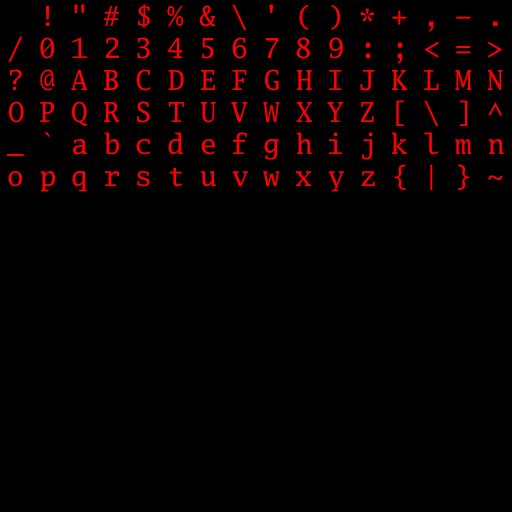
\includegraphics[width=0.5\textwidth]{images/font_texture.png}
	\caption{Przykładowa tekstura dla czcionki Go-Mono \cite{GOMONOFONT} (opracowanie własne)}
	\label{font_texture}
\end{figure}

\subsubsection{Zasób materiału \textit{asset\_material}}
Zasób materiału \textit{asset\_material} reprezentuje parametry używanego podczas renderowania powierzchni
prymitywów przy pomocy następujących parameterów:
\begin{itemize}
	\item \textit{baseColorFactor}: współczynnik koloru podstawowego (vec4);
	\item \textit{metallicFactor}: współczynnik metaliczności zakres, $\left[0,1\right]$;
	\item \textit{roughnessFactor}: współczynnik chropowatości $\left[0,1\right]$;
	\item \textit{metallicRoughnessTexture}: tekstura metaliczności-chropowatości, opcjonalna;
	\item \textit{normalMapTexture}: mapa normalnych, opcjonalna.
\end{itemize}

\subsubsection{Zasób tekstury \textit{asset\_texture}}
Zasób tekstury \textit{asset\_texture} reprezentuje próbkowalny obraz i składa się z zasobu obrazu oraz zasobu próbnika.

\subsubsection{Zasób obrazu \textit{asset\_image}}
Zasób obrazu \textit{asset\_image} zawiera dane obrazu w postaci nieskompresowanej bitmapy.
Bitmapa to prostokątna tablica pikseli opisywana przez następujące parametry:
\begin{itemize}
	\item szerokość i wysokość (uint32\_t);
	\item liczba ścian: domyślnie 1 ściana, 6 ścian dla tekstur sześciennych (uint32\_t);
	\item liczba kanałów: specyfikuje liczbę komponentów i tym samym rozmiar piksela, jeden kanał jest reprezentowany przez jeden bajt (uint32\_t).
\end{itemize}

\subsubsection{Zasób próbnika \textit{asset\_sampler}}
Zasób próbnika \textit{asset\_sampler} reprezentuje parametry używane do stworzenia próbnika obrazu:
\begin{itemize}
	\item \textit{magFilter}: filtr pomniejszający (VkFilter),
	\item \textit{minFilter}: filtr powiększający (VkFilter),
	\item \textit{addressModeU}: tryb adresowania współrzędnych tekstur poza przedziałem $\left[0,1\right]$ dla osi X (VkSamplerAddressMode),
	\item \textit{addressModeV}: tryb adresowania współrzędnych tekstur poza przedziałem $\left[0,1\right]$ dla osi Y (VkSamplerAddressMode),
\end{itemize}

\subsubsection{Potok zasobów asset\_pipeline}
Potok zasobów składa się z dwóch części:
\begin{itemize}
	\item narzędzia wiersza poleceń \textit{asset\_pipeline},
	\item skryptu Python \textit{asset\_pipeline}.
\end{itemize}

Skrypt skanuje podkatalog z zasobami wejściowymi i wywołuje narzędzie z argumentami będącymi ścieżką zasoby wejściowego rodzajem konwertowanego zasobu wyjściowego.
Przykładowo poniższy potok zasobów wywołuje narzędzie 5 razy tworząc pustą konfigurację globalną oraz pustą bazę zasobów wypełnioną zasobem skybox, zasobem czcionki Go-Mono oraz zasobami składającymi się na scenę Sponza opisanej plikiem glTF:
\lstset{language=verbatim}
\begin{lstlisting}[caption={Komeny wywoływane przez przykładowy potok zasobów},captionpos=b]
asset_pipeline empty_config
asset_pipeline empty_assets
asset_pipeline cubemap "skybox1" "/home/user/repo/cmake-build-debug/assets/cubemap/skybox1" png
asset_pipeline font "Go-Mono" "/home/sszczyrb/repo/cmake-build-debug/assets/font/Go-Mono.ttf"
asset_pipeline gltf "sponza" "/home/user/repo/cmake-build-debug/assets/gltf/sponza"
\end{lstlisting}

\subsection{Vulkan}

// TODO Vulkan to moduł zawierajacy 

\subsubsection{Jednostka shader}
Obiekt \textit{shader} reprezentuje pojedynczy shader i jest odpowiedzialny za kompilację ich do formy używalnej przez Vulkan.

Obiekt składa się z następujących elementów:
\begin{itemize}
	\item typ shadera,
	\item kod źródłowy GLSL,
	\item kod bajtowy SPIR-V,
	\item moduł shadera,
	\item obiekt \textit{shader\_reflect}.
\end{itemize}

Typ shadera zależy od tego, dla którego etapu potoku graficznego jest on przeznaczony.
Wspierane są dwa typy: wierzchołków i fragmentów.

Kod źródłowy GLSL must być znany podczas tworzenia - jest on uzyskiwany poprzez użycie obiektu \textit{shader\_generator}.

Kod bajtowy SPIR-V jest uzyskiwany poprzez kompilację kodu źródłowego GLSL biblioteką \textit{shaderc}.
Jej użycie ilustruje poniższy kod:
\lstset{language=C}
\begin{lstlisting}[caption={Kompilacja kodu źródłowego GLSL biblioteką \textit{shaderc}},captionpos=b]
shaderc_compiler_t compiler = shaderc_compiler_initialize();

shaderc_compile_options_t options = shaderc_compile_options_initialize();
shaderc_compile_options_set_target_env(options, shaderc_target_env_vulkan, 0);

const char *glslCode = ...;
size_t glslLen = strlen(glslCode);
shaderc_shader_kind shaderType = ...;
const char *inputFileName = "shader";
const char *entryPointName = "main";
shaderc_compilation_result_t result = shaderc_compile_into_spv(
compiler, glslCode, glslLen,
shaderType, inputFileName, entryPointName, NULL);
shaderc_compile_options_release(options);

if (shaderc_result_get_num_errors(result)) {
	const char *errorMsg = shaderc_result_get_error_message(result);
	panic("compilation error: %s\n", errorMsg);
}

size_t spvSize = shaderc_result_get_length(result);
uint32_t *spvCode = (uint32_t *)malloc(spvSize);
core_memcpy(spvCode, (uint32_t *)shaderc_result_get_bytes(result), spvSize);

shaderc_result_release(result);
shaderc_compiler_release(compiler)
\end{lstlisting}

Moduł shadera jest on uzyskiwany poprzez kompilację kodu bajtowego SPIR-V funkcją vkCreateShaderModule(), który jest też używany do uzyskania obiektu \textit{shader\_reflect}.

\subsubsection{Jednostka shader\_reflect}
Obiekt \textit{shader\_reflect} reprezentuje mechanizm refleksji shadera pozwalający na badanie jego struktury.
Operuje on na kodzie bajtowym SPIR-V i jest on używany podczas testów oraz do logowania informacji debugujących.

\subsection{Scena}

Moduł sceny jest odpowiedzialny za konwersję sceny z wysokopoziomowej formy używanej przez bazę zasobów do niskopoziomowej formy łatwo używalnej przez renderer do wyemitowania polecenia rysowania pośredniego.

Implementacja została zainspirowana techniką modelowania hierarchicznego opracowana w firmie Nvidia \cite{ADVANCEDSCENEGRAPH}.

Scena jest opisywana przy pomocy grafu sceny, którego węzeł zawieraja zasób prymitywu, lokalną trasformację przestrzeni świata oraz węzły potomne.
W tradycyjnym podejściu do modelowania hierarchicznego 
 znajdują się w  przy użyciu grafu sceny
// HIRO

Obiekty biorące udział w procesie konwersji sceny wraz z przepływem danych są przedstawione na poniższym diagramie:
\begin{figure}[H]
	\centering
	\begin{tikzpicture}[node distance=0.5cm]
		\tikzstyle{entity} = [rectangle, minimum width=3cm, minimum height=0.5cm,text centered, draw=black]
		\tikzstyle{flows} = [thick,->,>=stealth]
		
		\node (scene_data) [entity] {scene\_data};
		\node (scene_graph) [entity, below = of scene_data] {scene\_graph};
		\node (scene_tree) [entity, below = of scene_graph] {scene\_tree};
		\node (renderer_cache) [entity, below = of scene_tree] {renderer\_cache};
		
		\node (scene_graph_node) [entity, right = of scene_graph] {scene\_graph\_node};
		\node (scene_graph_node_dots) [right = 1mm of scene_graph_node] {...};
		\node (scene_tree_node) [entity, right = of scene_tree] {scene\_tree\_node};
		\node (scene_tree_node_dots) [right = 1mm of scene_tree_node] {...};
		
		\node (renderer_cache_primitive_element) [entity, below = of renderer_cache] {renderer\_cache\_primitive\_element};
		\node (renderer_cache_primitive_element_dots) [right = 1mm of renderer_cache_primitive_element] {...};
		\node (renderer_cache_camera_element) [entity, below = of renderer_cache_primitive_element] {renderer\_cache\_camera\_element};
		\node (renderer_cache_camera_element_dots) [right = 1mm of renderer_cache_camera_element] {...};
		\node (renderer_cache_direct_light_element) [entity, below = of renderer_cache_camera_element] {renderer\_cache\_direct\_light\_element};
		\node (renderer_cache_direct_light_element_dots) [right = 1mm of renderer_cache_direct_light_element] {...};
		\node (renderer_cache_skybox_element) [entity, below = of renderer_cache_direct_light_element] {renderer\_cache\_skybox\_element};
		\node (renderer_cache_skybox_element_dots) [right = 1mm of renderer_cache_skybox_element] {...};
		\node(renderer_cache_elements)[draw,dotted,fit=(renderer_cache_primitive_element) (renderer_cache_camera_element) (renderer_cache_direct_light_element) (renderer_cache_skybox_element) (renderer_cache_direct_light_element_dots)] {};
		
		\node (vkCmdDrawIndexedIndirect) [entity, right = of renderer_cache_elements] {vkCmdDrawIndexedIndirect()};
		
		\draw [flows] (scene_data) edge[out=-90,in=90] (scene_graph);
		\draw [flows] (scene_graph) edge[out=180,in=180] (renderer_cache);
		\draw [flows] (scene_graph) edge[out=-90,in=90] (scene_tree);
		\draw [flows] (scene_graph) edge[] (scene_graph_node);
		\draw [flows] (scene_graph_node) edge[] (scene_tree_node);
		\draw [flows] (scene_tree) edge[out=-90,in=90] (renderer_cache);
		\draw [flows] (scene_tree) edge[] (scene_tree_node);
		\draw [flows] (renderer_cache) edge[] (renderer_cache_elements);
		\draw [flows] (renderer_cache_elements) edge[] (vkCmdDrawIndexedIndirect);
		// HIRO nodes
		
	\end{tikzpicture}
	\caption{Obiekty biorące udział w procesie konwersji sceny wraz z przepływem danych (opracowanie własne)}
	\label{scene_process}
\end{figure}

\subsubsection{Dane sceny scene\_data}
Obiekt \textit{scene\_data} reprezentuje dane sceny wczytane z bazy zasobów. Jest one używany przez moduł sceny do konstrukcji grafu sceny \textit{scene\_graph}.

Obiekt utrzymuje on dla każdego typu obiektu zasobu osobną listę dwukierunkową zawierającą wszystkie obiekty używane przez scenę oraz ich domyślne warianty. Przykładowo domyślny obraz \textit{asset\_image} to obraz 2D o rozmiarze 1x1 mający 4 8-bitowe komponenty o wartości 255.

Wśród wszystkich obiektów zasobów składających się na dane sceny dodatkowo wyróżnia się:
\begin{itemize}
	\item węzły główne: używane jako punkty początkowe podczas tworzenia grafu sceny,
	\item używany skybox: może być zmieniony w konfiguracji zasobów,
	\item aktywna czcionka: sterowana konfiguracją globalną,
	\item domyślna kamera: używana w przypadku braku węzła z przypisaną kamerą.
\end{itemize}

Metody \textit{serialize()} i \textit{deserialize()} podobnie jak analogiczne metody obiektów zasobów pozwalają na zapis i odczyt danych sceny do bazy zasobów.

Metoda \textit{create\_with\_gltf\_file()} jest wywoływane wyłącznie przez potok zasobów.
Jej wejściem jest nazwa tworzonej sceny i ścieżka do katalogu zawierającego zasób 3D w formacie \textit{glTF} wraz z konfiguracją zasobów.
Oba zasoby wejściowe są parsowane przy użyciu biblioteki \textit{cgltf} i obiektu \textit{config}.
Wynik parsowania jest używany do stworzenia i wypełnienia danych sceny.
Ta metoda wraz z metodą \textit{serialize()} stanowi główną częścią potoku zasobów - obiekt stworzony na podstawie zasobów wejściowych jest serializowany do zasobu wyjściowego (bazy zasobów).

Metoda \textit{create\_with\_asset\_db()} jest wywoływana w czasie wykonywania i wczytuje dane sceny o żądanej nazwie z bazy zasobów.

\subsubsection{Graf sceny scene\_graph}
Obiekt \textit{scene\_graph} reprezentuje
// HIRO

\subsubsection{Drzewo sceny scene\_tree}
Obiekt \textit{scene\_tree} reprezentuje
// HIRO

\subsection{Renderer}

// TODO Renderer to moduł zawierajacy 

// HIRO renderer\_cache

// HIRO Stan renderowania renderer\_state

// HIRO Graf renderowania render\_graph

// HIRO renderer